\chapter{Resultados Experimentais}\label{chap6}


Esse capítulo apresenta os experimentos conduzidos com AEH-ETAA para avaliar a abordagem proposta. Foram conduzidos experimentos teóricos e práticos. As seções seguintes apresentam esses experimentos e discutem os resultados obtidos.
% This section presents experiments conducted with HEA-TaSDAP to evaluate the proposed approach. We conducted two types of experiments: theoretical and practical ones. The central idea of this section is to compare the proposed scheduling approach with existing solutions that can be used to schedule workflows in clouds. It is worth mentioning that all schedules used in this section for experiments and all optimization code are available in a BitBucket Git repository (\url{https://bitbucket.org/danielcmo/hea-tasdap}). 



\section{Experimentos Teóricos}

O AEH-ETAA foi comparado em termos de qualidade de solução  e tempo de execução com: (i) as soluções dadas pela formulação matemática IP-ETAA (resolvida com CPLEX $12.5.1$); (ii) A heurística MinMin \cite{minmin}; e (iii) a heurística HEFT \cite{HEFT}. As heurísticas MinMin e HEFT foram escolhidas pois executam em tempo polinomial, produzem escalonamentos eficientes e foram utilizados na comparação de diversos trabalhos relacionados \cite{Rahman2007, Lopez, Yu2006}.

% 	We firstly evaluate HEA-TaSDAP, in terms of  quality of solution and execution time, by comparing it with: (i) the solutions given by mathematical formulation TaSDAP-IP (solved with CPLEX $12.5.1$); (ii) the MinMin-Task Scheduling Heuristic (MinMin-TSH) \cite{MINMIN}; and (iii) the Heterogeneous Earliest Finish Time (HEFT) \cite{HEFT}.  We have chosen MinMin-TSH and HEFT because these heuristics run in polynomial time, produce efficient schedules and have been used as baselines in related works  \cite{Rahman2007,Lopez, Yu2006}. 
	
	
Os testes foram realizados em um computador com processador Intel Core i7-3770 CPU $3,40$ GHz com 12GB memoria, executando o Ubuntu $14.04$. O algoritmos AEH-ETAA, MinMin e HEFT foram implementados com C++, e compilados com o G++ versão $5.3.0$.

% 	Tests were run in a computer with a processor Intel Core i7-3770 CPU 3.40 GHz with 12Gb memory running Ubuntu $14.04$. The HEA-TaSDAP, MinMin-TSH and HEFT were implemented with C/C++, and compiled with g++ version $5.3.0$.
	
Nesses experimentos, foram utilizados dois tipos de instâncias sintéticas. O primeiro tipo, usado na comparação entre o AEH-ETAA e IP-ETAA (Subseção \ref{ssec:CompEX}), é composto por soluções geradas randomicamente, variando o número de tarefas, a quantidade de arquivos e o modelo de representação dos \textit{workflows}. O segundo, utilizado na Subseção \ref{ssec:compT}, foi gerado pelo \textit{Workflow Generator} \cite{Silva2014} (\url{https://confluence.pegasus.isi.edu/display/pagasus/WorkflowGenerator}), uma aplicação que gera \textit{workflows} sintéticos utilizados na avaliação de diversos algoritmos de escalonamento. O \textit{Workflow Generator} utiliza dados coletados de execuções reais de WfCs executados em \textit{grids} e ambientes de nuvem e, por conta disso, apresenta uma boa acurácia em relação às características reais dos \textit{workflows}.

% 	We use two types of synthetic instances in these experiments. The first one, used in the comparison  between HEA-TasDap and TaSDAP-IP (Subsection \ref{ssec:CompEX}), was randomly generated varying the number of tasks, data files and representations of workflows, as explained later. The second type, used in Subsection \ref{ssec:compT}, was generated by the Workflow Generator \cite{Silva2014}  (\url{https://confluence.pegasus.isi.edu/display/pegasus/WorkflowGenerator}). This application generates instances of workflow executions for evaluation of algorithms and systems on a range of workflow sizes. All data within these synthetic workflows is gathered from real executions of scientific workflows on the grid and in the cloud from the Pegasus' team in ISI @ University of Southern California.
	
A metaheurística AEH-ETAA foi executada com uma população de 50 indivíduos e o critério de parada foi definido como 100 iterações sem melhorias.

% 	The metaheuristic HEA-TaSDAP was executed with a population of 50 individuals and the stopping criterion was satisfied after 100 iterations without improvement. Concerning  the other parameters, the algorithm uses the ones defined in Section \ref{sec:HEA}.  It is worth mentioning that all parameters were adjusted empirically after several tests.
	


\subsection{Comparação do AEH-ETAA com a Abordagem Exata IP-ETAA}\label{ssec:CompEX}

O AEH-ETAA e o IP-ETAA foram avaliados utilizando um conjunto de 12 instâncias divididas em 4 grupos de acordo com o seus tamanhos. Para cada grupo, três instâncias diferentes foram geradas variando o número de tarefas, arquivos, e a representação do \textit{workflow}. Dois ambientes computacionais foram definidos para a simulação, com 3 e 5 MVs. O tamanho dos arquivos (MB) e tempo de execução das tarefas (segundos) foram definidos aleatoriamente entre 0,1 e 100. Uma capacidade de armazenamento de 10 GB foi definida e enlaces de 5, 10 e 15 MB/s foram utilizados. Por fim, o valor de \textit{slowdown} das máquinas foi configurado entre 0,01 e 1. A Tabela \ref{tabletoy} mostra a quantidade de tarefas e arquivos para cada instância gerada. Além disso, a estrutura básica do \textit{workflow} de cada uma delas é apresentada de acordo com a classificação feita por Bharathi \textit{at al.} \cite{Bharathi2008}. A Figura \ref{fig:structure} apresenta essa classificação e as estruturas dos \textit{workflows}.

% 	HEA-TaSDAP and TaSDAP-IP were evaluated using a set of 12 random instances divided into 4 groups according to their sizes. For each group, three different instances were generated by varying the number of tasks, files, and the representation of the workflow. Two computational environments were defined for simulation, with 3 and 5 VMs. File sizes (MB) and the process execution time (seconds) were randomly set between 0.1 and 100. The storage capacity of 1TB has been set, and the transfer link rates were 5, 10 and 15 MB/s. Finally, the slowdown of the machines were set between 0.01 and 1. Table \ref{tabletoy} shows the amounts of tasks and files for each generated instance. In addition, the basic workflow structures found on them are presented according to the classification made by Bharathi \textit{et al.} \cite{Bharathi2008}.

\begin{table}[!ht]

    \begin{center}
        \caption{Descrição das Instâncias Utilizadas na comparação com a formulação matemática.}
        \label{tabletoy}
        
         \begin{tabular}{|c |c |c |c |}
            \hline
            \textbf{\textbf{Referência}} & \textbf{Estrut. Básica} & \textbf{Núm. tarefas} & \textbf{Núm. arquivos}\\
            \hline\hline
                5A           & Processamento                            & 2     & 3\\
                5B           & Processamento e agregação de dados       & 2     & 3\\
                5C           & Agregação de dados                       & 1     & 4\\
                \hline
                7A          &   Agregação e redistribuição de dados     & 2     & 5\\ 
                7B          &   Processamento                           & 3     & 4\\
                7C          &   Agregação de dados e \textit{pipeline}  & 3     & 4\\
                \hline
                10A         & Agregação de dados                        & 4  & 6\\
                10B         & Redistribuição de dados                   & 3  & 7\\
                10C         & Distribuição de dados e \textit{pipeline} & 3  & 6\\
                \hline
                15A         & Agregação e distribuição de dados         & 5  & 10\\
                15B         & Distribuição de dados e \textit{pipeline} & 4  & 11\\
                15C         & Agregação e distribuição de dados         & 5  & 10\\                  
             \hline
         \end{tabular}
    \end{center}
\end{table}


\begin{figure}[H]
\centering
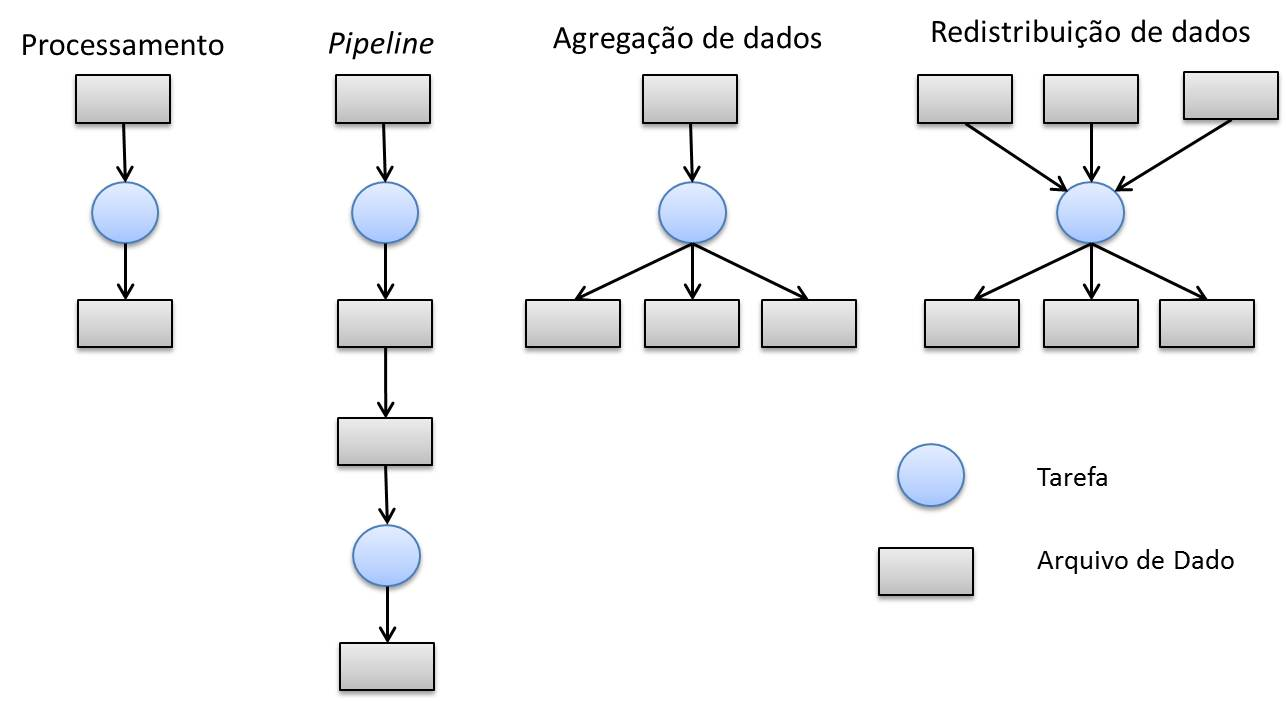
\includegraphics[width=.6\linewidth]{figure/structure.jpg}
\caption{Estruturas básicas dos \textit{workflows} (adaptado de \cite{Bharathi2008}).}
\label{fig:structure}
\end{figure}


	 
A Tabela \ref{teorico} apresenta os resultados obtidos pela abordagem exata e pela metaheurística AEH-ETAA. A primeira coluna identifica as instâncias e nas duas colunas seguintes são apresentados os resultados obtidos pelo AEH-ETAA: \textit{makespan} obtido e tempo de execução do algoritmo. Em seguida, nas duas próximas colunas, são apresentadas as informações referentes a abordagem exata. Por fim, a diferença percentual entre a solução dada pela metaheurística e pela abordagem exata é mostrada. O valor de \textit{makespan} apresentados para AEH-ETAA representam a média de cinco execuções. Além disso,  como os valores de desvio padrão foram iguais a zero para quase todas as instâncias,  com exceção das instâncias $15B\_m3, 15B\_m5$ e $15A\_m5$ que foram menos de $0,6\%$, essa informação não é apresentada.
	 
% 	 Table \ref{teorico} summarizes the results obtained by exact approach and the HEA-TaSDAP metaheuristic. The first column identifies the instance. The following two columns present the results obtained by HEA-TaSDAP: makespan and the execution time to obtain the solution. Following, the next 2 columns present the same results for the exact approach. Finally, the last column, shows the gap between the solutions given by HEA-TaSDAP and the exact approach (mathematical formulation). The values shown for HEA-TaSDAP are averages of five executions. The standard deviations were zero for almost all instances, except $15B\_m3$, $15B\_m5$ and $15A\_m5$, which were less than $0.6$. 


Analisando a Tabela \ref{teorico} pode-se observar que para todas as instâncias avaliadas o AEH-ETAA obteve soluções com uma diferença percentual baixa (média $1,1\%$), com tempos de execução  significativamente menores em relação à formulação matemática resolvida com o CPLEX, em média $1,5$s contra $12.640,3$s, respectivamente. Além disso, o CPLEX não foi capaz de encontrar soluções viáveis para as instancias $10A\_m5$ e $15C\_m5$ dentro de um limite de 24 horas.
Ademais, na instância $15C\_m3$, o CPLEX não foi capaz de encontrar a soluções ótima. Embora esses resultados sejam encorajadores, o AEH-ETAA também foi avaliado com outras heurísticas utilizando outras instâncias, como apresentado nas próximas seções.
	 
\begin{table}[H]
\begin{minipage}{\textwidth}   
    \begin{center}
            \caption{Resultados da metaheurística AEH-ETAA e da formulação matemática utilizando o CPLEX.}
        \label{teorico}        
          \begin{tabular}{|c|r|r|r|r|r|}
            \hline
            \multirow{1}{*}{\textbf{Instâncias}} & \multicolumn{2}{|c|}{\textbf{AEH-ETAA}} & \multicolumn{2}{|c|}{\textbf{Formulação Matemática}} & \multirow{1}{*}{\textbf{Dif. Percentual}}\\
\cline{2-5}
            \hline\hline          
5A\_m3	&	10,0	&	0,83    &	10,0	&	 4,2    &	0,0	\\
5B\_m3	&	11,0	&	0,79    &	11,0	&	 14,0   &	0,0	\\
5C\_m3	&	13,0	&	0,71    &	13,0	&	 2,8    &	0,0	\\
7A\_m3	&	21,0	&	0,96    &	21,0	&	140,8	&	0,0	\\
7B\_m3	&	16,0	&	1,17    &	16,0	&	 7,3	&	0,0	\\
7C\_m3	&	14,0	&	1,11	&	14,0	&	105,0	&	0,0	\\
10A\_m3	&	21,0	&	1,80	&	21,0	&	1644,6	&	0,0	\\
10B\_m3	&	12,0	&	1,74	&	12,0	&	21,4	&	0,0	\\
10C\_m3	&	21,0	&	1,22	&	21,0	&	316,7	&	0,0	\\
15A\_m3	&	16,0	&	2,47	&	16,0	&	2606,6	&	0,0	\\
15B\_m3	&	11,4	&	3,01	&	11,0	&	600,9	&	3,6	\\
15C\_m3\footnote{\label{1footnote} O CPLEX não foi capaz de encontrar solução viável para a instância.}&	19,2	&	2,42	&	94,0	&	86395,5	&	\textbf{--}	\\
5A\_m5	&	10,0	&	0,90	&	10,0	&	14,4	&	0,0	\\
5B\_m5	&	 9,0	&	0,50	&	 9,0	&	462,6	&	0,0	\\
5C\_m5	&	10,0	&	0,75	&	10,0	&	 9,0	&	0,0	\\
7A\_m5	&	27,0	&	0,97	&	27,0	&	1836,4	&	0,0	\\
7B\_m5	&	26,0	&	1,26	&	26,0	&	21,0	&	0,0	\\
7C\_m5	&	16,0	&	1,09	&	16,0	&	2426,9	&	0,0	\\
10A\_m5\footref{1footnote}&	25,0	&	1,58	&	\textbf{--}	    &	86489,2	&	\textbf{--}	\\
10B\_m5	&	14,0	&	1,75	&	13,0	&	103,0	&	7,6	\\
10C\_m5	&	47,6	&	1,88	&	47,0	&	7353,5	&	1,2	\\
15A\_m5	&	16,0	&	2,64	&	16,0	&	15783,9	&	0,0	\\
15B\_m5	&	11,0	&	2,97	&	10,0	&	10764,3	&	10,0	\\
15C\_m5\footref{1footnote}&	20,0	&	2,49	&	\textbf{--}	    &	86243,0 &  \textbf{--}	\\
\hline
Média	&	17,4	&	1,5	    &	20,2	&	12640,3	&	1,1	\\
             \hline
         \end{tabular}
    \end{center}
    \end{minipage}
\end{table}
	 
	 

\subsection{Comparação do AEH-ETAA com as Heurísticas  HEFT e MinMin}\label{ssec:compT}

Para comparar a performance e a qualidade dos resultados do AEH-ETAA com as heurísticas HEFT e MinMin, as instâncias sintéticas produzidas pelo \textit{workflow generator} baseadas nos \textit{workflows} Montage, Cybershake, Epigenomics e Inpiral  \cite{juve2406180} foram escolhidas. Cada instância tem as seguintes informações: (i) um DAG representando o \textit{workflow}; (ii) o tempo de execução de cada tarefa em relação a uma máquina com capacidade de processamento conhecida; e (iii) o tamanho de cada arquivo de entrada e de saída. A Tabela \ref{workflowCharacteristics} apresenta um resumo das principais características de cada um destes \textit{workflows}. Para o ambiente de execução, foram consideradas as características (largura de banda, capacidade de armazenamento e processamento) das MVs oferecidas pela Amazon EC2. Foram utilizadas 4 MVs: 1 m3.medium (1 vCPU Intel Xeon E5-2670 v2); 1 m3.large (2 vCPU Intel Xeon E5-2670 v2); 1 m3.xlarge (4 vCPU Intel Xeon E5-2670 v2); 1 m3.2xlarge (2 vCPU Intel Xeon E5-2670 v2). Portanto, embora a avaliação seja teórica, os dados utilizados na descrição dos \textit{workflows} e das MVs foram adquiridos com base em cenários reais. 


% In order to compare the performance and the quality of the results of  HEA-TaSDAP, HEFT and  MinMin-TSH, the aforementioned synthetic  workflows  produced by workflow generator: Montage, Cybershake, Epigenomics and Inspiral workflows \cite{Juve2406180} were chosen.  Each instance (workflow) has the following corresponding information: (i) a Direct Acyclic Graph representing  tasks  and data files of the workflow; (ii) execution time  of each task in a machine with known processing capacity; and (iii) size of each  input and output data file.   Table \ref{workflowCharacteristics} shows the main characteristics of each workflow.

\begin{table}[!ht]
    \begin{center}
        \caption{Atributos dos \textit{workflows} utilizados na avaliação teórica entre o AEH-ETAA, HEFT e MinMin (Adaptado de \cite{Szabo2013}).}
        \label{workflowCharacteristics}
        
         \begin{tabular}{|c |c |c |c |}
            \hline
            \multirow{2}{*}{\textbf{Workflow}} & \multirow{1}{*}{\textbf{Tipo}} & \textbf{Núm. de tarefas} & \textbf{Núm. de arquivos}\\
            & \textit{ I/O; Memória; CPU}    &\textbf{por instâncias}& \textbf{dinâmicos e estáticos}\\
            \hline\hline
    Cybershake  & Baixo; Baixo; Médio     & 30; 50; 100            & 49; 79; 154 \\
	Epigenomics & Baixo; Médio; Alto      & 24; 47; 79; 100; 127   & 38; 71; 119; 152; 192;  \\
	Montage	    & Alto; Baixo; Baixo      & 25; 50; 100            & 38; 53; 93 \\
	Inspiral    & Baixo; Médio; Alto      & 30; 50; 100            & 47; 77; 151  \\
             \hline
         \end{tabular}
    \end{center}
\end{table}




% We also considered the characteristics of the VMs from Amazon EC2 cloud environment. So, although we are theoretically evaluating the algorithms, the used data (structure of workflows and VMs characteristics) were acquired from real scenarios. The used cloud environment is composed by 4 VMs: 1 m3.medium (1 vCPU Intel Xeon E5-2670 v2); 1 m3.large (2 vCPU  Intel Xeon E5-2670 v2); 1 m3.xlarge (4 vCPU Intel Xeon E5-2670 v2); 1 m3.2xlarge (8 vCPU Intel Xeon E5-2670 v2).  We also considered the following information about  each VM: (i) network bandwidth; (ii) storage capacity; and (iii) processing capacity. 

O tempo de execução das tarefas é definido como o produto do \textit{tempo base} pelo valor de \textit{slowdown} da MV que executará a tarefa. O valor de \textit{slowdown} é definido como $\frac{P_B}{P_{mv_{j}}}$, onde $P_B$ é a capacidade de processamento da máquina usada na estimativa do \textit{tempo base}, e $P_{mv_{j}}$ é a capacidade de processamento da máquina virtual $mv_j$ usada no experimento. Portanto, o \textit{slowdown} dá a variação da capacidade de processamento de uma MV em relação a máquina utilizada para calcular o \textit{tempo base} da tarefa. Neste experimentos, o \textit{tempo base} e a capacidade do processamento da máquina $P_B$ foram obtidos a partir das instâncias dadas pelo \textit{Workflow Generator}, enquanto $P_{mv_{j}}$ é a capacidade de processamento da máquina virtual oferecido pela Amazon EC2.

% It is worth mentioning that the execution time of a task is defined as the product between a basis time and the machine slowdown where it will be executed. A machine slowdown is defined  as  $\frac{P_B}{P_{m_{j}}}$, where $P_B$ is the  processing capacity of the machine  used to calculate the basis time, and   $P_{m_{j}}$  is the  processing capacity of the virtual machine of our experiment. So,  the  slowdown represents the processing capacity of a virtual machine when compared with the  machine used to calculate the basis time.  In our experiments, the basis time and the processing capacity $P_B$  were obtained from  instances of the Workflow Generator, while $P_{m_{j}}$  is the  processing capacity of the virtual machine  from  Amazon EC2. The parameter of transfer rate was estimated through practical experiments using the tool Iperf, available in \url{https://iperf.fr}.

A Tabela \ref{teoricoSintetico} apresenta o \textit{makespan} obtido pela média de 5 execuções, o desvio padrão relativo (RSD) e o tempo de execução do AEH-ETAA. Também são apresentados o \textit{makespan} obtido com as heurísticas MinMin e HEFT. Como essas heurísticas são determinísticas, os resultados sempre serão os mesmos para entradas semelhantes, os valores de \textit{makespan} não são médias de execuções e sim o valor obtido com uma única execução. Além disso, o tempo de execução do MinMin e do HEFT não são apresentados, pois eles são insignificantes (menos que 1 minuto).


Como pode ser visto na Tabela \ref{teoricoSintetico} a metaheurística AEH-ETAA supera ambos os algoritmos comparados. De fato, esses resultados são esperados, já que variações das soluções dadas pelo MinMin e pelo HEFT são utilizadas pela metaheurística na geração da população inicial. Porém, vale notar que houve uma melhora na qualidade dos valores de \textit{makespan} em todos os casos de teste, com um tempo de execução aceitável (menos de 9 minutos no pior caso). O AEH-ETAA apresentou uma melhora média de $22,72\%$ em relação ao MinMin e $11,15\%$ em relação ao HEFT.

% Table \ref{teoricoSintetico} presents the makespan (the average of 5 executions), Relative Standard Deviation (RSD) and the execution time of HEA-TaSDAP. It also presents the makespan of MinMin-TSH and HEFT, and since they are deterministic heuristics, the result is always the same for each execution of the algorithm. The execution times of MinMin-TSH and HEFT are not presented, since they are negligible (less than 1 minute). Note that, HEA-TaSDAP outperforms both MinMin-TSH and HEFT algorithms.

% In fact, these results were already expected, since variations of solutions given by MinMin-TSH and HEFT are used in initial population. It worth noticing that with our proposal we improved the quality of the makespan in all cases and with a acceptable run time (less than 9 minutes in the worst case). The HEA-TaSDAP showed an average improvement of 22.72\% in relation of MinMin-TSH and 11.15\% in relation of HEFT.


\begin{table}[H]
\small
\begin{center}
\caption{Resultados da comparação entre AEH-ETAA, HEFT e MinMin.}
\label{teoricoSintetico}
\begin{tabular}{|c|r|r|r|r|r|}\hline 
\multirow{2}{1cm}{\textbf{Inst}.} & \multicolumn{1}{|c|}{\textbf{MinMin}} & \multicolumn{1}{|c|}{\textbf{HEFT}} & \multicolumn{3}{|c|}{\textbf{AEH-ETAA}} \\    
\cline{2-6}  
                &\textit{	Makesp. (min)} & \textit{Makesp. (min)} &	\textit{Makesp. (min)} & \textit{RSD}	 & \textit{Exec. (min)}\\
\hline
\hline
Cybershake30    &	11,98	       & 11,28          &   10,25              & 0,0019    &	0,39          \\
Cybershake50    &	14,88	       & 16,65	        &   12,46	       & 0,0264    &	2,19          \\
Cybershake100   &   26,93	       & 28,08	        &   14,52	       & 0,0261    &    8,11          \\
Genome.3510     &	530,88         & 469,38         &	444,91         & 0,0109    &	4,05          \\
Genome.7020     &	923,46         & 865,45         &	833,98         & 0,0004    &	6,79          \\
Epigenomics24   &	67,36          & 57,30          &	55,80          & 0,0000    &    0,03          \\
Epigenomics46   &	119,95         & 104,07         &	99,27          & 0,0140    &    0,48          \\
Epigenomics100  &   1,004,23           & 916,73         &	889,65         & 0,0001    &    4,02          \\
Montage25	&   1,81               & 1,16           &	0,95           & 0,0242    &	0,05          \\
Montage50       &   3,06               & 2,08           &	1,88           & 0,0036    &	0,10          \\
Montage100	    &   5,31           & 4,66           &	3,93           & 0,0038    &	3,33          \\
Inspiral30	    &   18,26          & 14,61          &	13,95          & 0,0014    &	0,17          \\
Inspiral50	    &   29,96          & 23,36          &	22,41          & 0,0005    &	0,79          \\
Inspiral100	    &   44,65          & 41,80          &	40,76          & 0,0036    &	1,55          \\
\hline
\end{tabular}
\end{center}
\end{table}	




\section{Avaliação do AEH-ETAA com \textit{Workflows} Reais}

Esta subseção apresenta a avaliação do AEH-ETAA usando um \textit{workflow} real de bioinformática. Para isso, o SGWfC SciCumulus foi escolhido para executar os escalonamentos. As seguintes seções apresentam o \textit{workflow} utilizado como estudo de caso, uma breve descrição do SGWfC usado e as modificações necessárias para realizar os testes, a configuração do ambiente e os resultados obtidos.

% This subsection presents the evaluation of the scheduling provided by HEA-TaSDAP using a real workflow from the bioinformatics domain. To achieve that, we have chosen the SWfMS SciCumulus to execute the schedule provided by HEA-TaSDAP. The following sections present the workflow used as case study, a brief description of the SWfMS used and the needed modifications, the environment configurations and the results achieved.

\subsection{SciPhy: Um \textit{workflow} para análises filogenéticas}

Vários tipos de experimentos de bioinformatica são baseados nos resultados das análises filogenéticas, como os experimetos farmacológicos, desenvolvimento de novas drogas, \textit{etc.} Uma análise filogenética tem o objetivo de produzir árvores filogênicas, que são estruturas que mostram as relações evolucionárias inferidas entre genes homólogos representados no genoma da espécie divergente. Gerenciar experimentos filogenéticos não é uma tarefa trivial, pois eles são \textit{compute-} e \textit{data-intensive}. Esses experimentos são baseados em \textit{pipelines} de programas científicos e, portanto, podem ser facilmente modelados como um WfC.

% This subsection presents the workflow used as a case study for a real workflow execution in this article. Many types of bioinformatics experiments are based on the outcome of a phylogenetic analysis, such as phamacophylogenomics experiments, development of new drugs, \textit{etc.} A phylogenetic analysis aims at producing phylogenetic trees, which are structures that show the inferred evolutionary relationships among homologous genes represented in the genomes of divergent species. Managing phylogenetic experiments is far from trivial, since they are compute- and data-intensive. As they are based on a pipeline of scientific programs, computational phylogenetic experiments can be modeled as a scientific workflow. 

O Sciphy \cite{ocana2011} é um dos \textit{workflows} existentes para análises filogenéticas. O \textit{workflow} executa análises com varredura de parâmetros, no qual o mesmo \textit{workflow} é executado para cada um dos arquivos de entrada. O \textit{workflow} é composto por quatro atividades principais: alinhamento de sequencias múltiplas (MSA, do inglês \textit{multiple sequence alignment}), conversor de sequências, busca pelo melhor modelo evolucionário, e construção das árvores filogenéticas. Essas atividades executam, respectivamente, as seguintes aplicações de bioinformática: programas MSA (MAFFT, KAlign, CLustalW, Muscle e ProbCons), ReadSeq, ModelGenerator, e RAxML.

% SciPhy \cite{ocana2011} is one of the existing workflows for phylogenetic analysis. SciPhy workflow is a parameter sweep analysis where the same workflow is executed for each input file in a given large input dataset. It is composed by four main activities: multiple sequence alignment (MSA), sequence conversion, search for the best evolutionary model, and construction of phylogenetic trees, and they respectively execute the following bioinformatics applications: MSA programs (MAFFT, Kalign, ClustalW, Muscle and ProbCons), ReadSeq, ModelGenerator, and RAxML.

Um grafo representando uma execução do SciPhy é apresentado na Figura \ref{fig:sciphy}. Cada círculo representa uma execução diferente da atividade em uma MV, e os retângulos representam os dados produzidos e consumidos.  A primeira atividade do SciPhy (que é associada a tarefa $tf_1, tf_5$ e $tf_n$) constrói MSAs individuais utilizando um dos cinco programas de MSA disponíveis - ClustalW, Kalign, MAFFT, Muscle, e ProbCons - com os parâmetros padrão. Cada programa MSA recebe um arquivo multifasta como entrada (contendo uma sequencia de DNA, RNA e aminoácidos - Mf1, Mf2 e Mfm), e produzem um MSA como saída (Ms1, Ms2 e Msm). Cada MSA é então convertido para o formato phylip pela segunda atividade (que é associada as tarefas $tf2, tf6$ e $tf_{n+1}$) para serem futuramento processadas. Após a conversão para o formato phylip (Rs1, Rs2 e Rsm), os arquivos são testados na terceira atividade para encontrar o melhor modelo evolutivo usando o ModelGenerator (associado as tarefas $tf_3, tf_6$, $tf_{n+2}$). Em seguida, o MSA individual, o MSA convertido e o modelo evolutivo são utilizados na quarta atividade (associada às tarefas $tf_4, tf_8$ e $tf_{n+3}$) para gerar as árvores filogenéticas (T1, T2 e Tm) usando o RAxML com 100 replicações \cite{raxml}. Consequentemente, podem ser obtidas várias árvores diferentes para cada um dos diferentes programas MSA e para os vários arquivos multifasta de entrada. Nos experimentos apresentados neste trabalho o MAFFT foi empregado como método de MSA.

\begin{figure}[!ht]
\centering
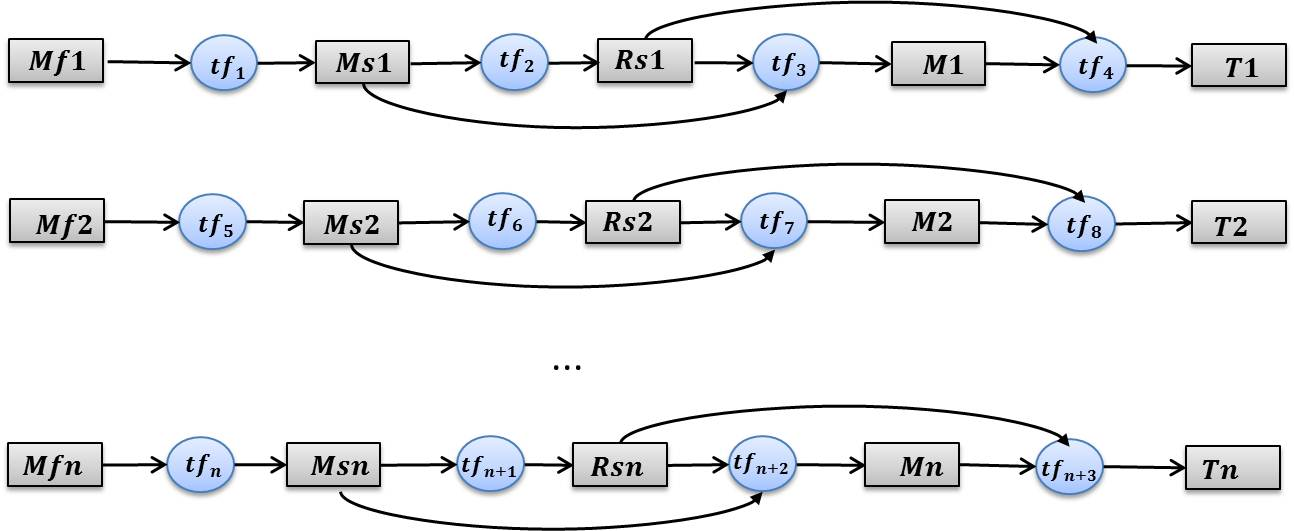
\includegraphics[width=0.8\linewidth]{figure/sciphy.jpg}
\caption{Um grafo representando uma única execução do Sciphy.}
\label{fig:sciphy}
\end{figure}

Como o objetivo é executar uma varredura de parâmetros no Sciphy, cada uma das atividades são executadas com diferentes arquivos de entrada contendo várias sequencias (arquivos multifasta) e, portanto, gerando diferentes tarefas. Cada uma dessas tarefas podem ser executadas em paralelo. Para mais informações sobre o Sciphy, consulte Ocanã \textit{et al.} \cite{ocana2011}.


\subsection{SGWfC SciCumulus}

O SGWfC SciCumulus oferece suporte para dois tipos de paralelismo: varredura de parâmetros \cite{Walker2007}; e paralelismo de dados \cite{Coutinho2010}. O gerenciador atua na distribuição, controle e monitoramento de execuções paralelas de WfCs executados em ambientes de nuvem, e é composto por 4 módulos:

\begin{enumerate}[I]
\item Camada Cliente: Os componentes desse módulo enviam os \textit{workflows} para serem executados na nuvem.
\item Camada de Distribuição: Gera e gerencia  atividades executáveis (tarefas) em uma ou mais MVs instanciadas em um ou mais ambientes de nuvem. 
\item Camada de Execução: É responsável pela execução dos programas invocados pelas atividade do \textit{workflow}, pela geração dos dados e pelo armazenamento dos dados de proveniência.
\item Camada de Dado: Essa camada é base de dados de proveniência, que armazena todos os dados de proveniência consumidos e gerados pela execução paralela do \textit{workflow}. 
\end{enumerate}

O SciCumulus oferece uma infraestrutura computacional mínima para suportar o paralelismo de \textit{workflows} com gerenciamento de dados de proveniência. Para os experimentos apresentados neste trabalho o escalonados do SciCumulus foi modificado. Na versão atual do SciCumulus, o escalonador é baseado em uma abordagem gulosa e dinâmica, chamada  aqui de Greedy-SC \cite{Oliveira2012}. No Greedy-SC sempre que uma máquina fica ociosa o escalonador é chamado para decidir qual será a melhor tarefa a ser executada naquela máquina. Essa é uma abordagem simples que apresenta bons resultados, especialmente quando há variações de performance nas MVs.

% SciCumulus provides the minimal computational infrastructure to support workflow parallelism with provenance management. 
% For the experiments presented in this article the scheduler of SciCumulus had to be modified. In the current and available version of SciCumulus, the scheduler is based on a greedy and dynamic approach. As a VM become idle, it requests a task and then the scheduler decides the best task to be executed in that VM on that specific moment. This is a simple approach and provides good solutions especially when we face performance variations in the VMs, but since it is based on a greedy algorithm, it is not guaranteed that the optimal solution is provided.

Na versão do SciCumulus usada neste experimento, o AEH-ETAA é invocado antes da execução do \textit{workflow}, e são fornecidas as informações das tarefas, dos arquivos e das MVs que formam o \textit{cluster} virtual na nuvem. Todos esses dados são consultados e resgatados dos dados de proveniência \cite{freire2008}. O AEH-ETAA cria então um plano de escalonamento que é retornado para o SciCumulus. O plano de escalonamento é carregado para uma tabela na base de dados, que é consultada pelo escalonar sempre que uma MV fica ociosa. Para mais informações sobre o SciCumulus consulte Oliveira \textit{et al.} \cite{oliveira2010}. 

% In the version of SciCumulus used in this experiment, the HEA-TaSDAP is invoked before each workflow execution. It is provided a list of tasks, the estimated execution time, the number of data files to be produced and consumed and the amount of VMs that are part of the virtual cluster in the cloud. All input data for HEA-TaSDAP is queried and retrieved from the provenance database \cite{freire2008}. HEA-TaSDAP then creates a scheduling plan that is returned to SciCumulus. This scheduled plan is loaded into a database table (since SciCumulus is database-oriented) and this table is queried by the scheduler every time a VM is idle. For more information about SciCumulus, please refer to Oliveira \textit{et al.} \cite{Oliveira2012}. As aforementioned, all scheduling plans provided by HEA-TaSDAP and the executable code will be available on the URL https://bitbucket.org/danielcmo/hea-tasdap. 

\subsection{Configuração do Ambiente}

Os experimentos práticos deste trabalho foram realizados no serviço de nuvem Amazon EC2. O Amazon EC2 é um dos provedores de nuvem comercial mais popular da atualidade, e inúmeras aplicações científicas e comerciais são executadas pelo serviço diariamente. No experimento apresentado neste trabalho foram considerados 2 tipos de MVs oferecidas pelo serviço: m3.small (1 VCpu e 3,75 GB memória RAM) e m3.2xlarge (8 VCpu e 30 GB de memória). As MVs foram definidas conforme as recomendações do GraspCC \cite{Coutinho201551}, uma técnica baseada do GRASP que dimensiona o ambiente de nuvem para WfCs. Segundo o algoritmo de dimensionamento, um ambiente composto por uma m3.small e duas m3.2xlarge seria suficiente para a execução do \textit{workflow} SciPhy.

% For the experiments executed in this article, we have deployed the 2 aforementioned versions of SciCumulus on top of Amazon EC2. Amazon EC2 is the most popular commercial cloud and many scientific and commercial applications are being deployed on it. Amazon EC2 provides several different types of VMs for deployment and use. In the experiments presented in this paper we have considered 2 types of VMs: m3.medium (1 CPU and 3.75 GB RAM) and m3.2xlarge (8 virtual CPU and 30 GB RAM). We have instantiated 1 m3.small and 2 m3.2xlarge following the recommendations of GraspCC \cite{Coutinho201551}, a GRASP-based approach for dimensioning the cloud environment for scientific workflows.


As MVs utilizadas tem como sistema operacional a distribuição Gnu/Linux Cent OS 7 (64 bits), e foram configuradas com os softwares e as bibliotecas necessárias para a execução das aplicações de bioinformática. As máquinas foram instanciadas na região de US East - N. Virginia e  seguem as regras de preço desta localidade. Além disso, as execuções do SciPhy foram realizadas em um único site da Amazon EC2. 

%  Each deployed VM presented in this article is based on the Linux Cent OS 7 (64-bit), and was configured with the necessary software and libraries, and the bioinformatics applications. All VMs were configured to be accessed using SSH. Additionally, these VMs are based on an a AMI image (ami-7e1a1716) that is also stored in the cloud as and SciCumulus creates the virtual cluster to execute the experiment based on this AMI. In terms of software, all VMs, no matter its type, execute the same programs and configurations. All VMs were deployed in the US East - N. Virginia location and follow the pricing rules of that locality. In addition, the executions of SciPhy were performed in a single site of the Amazon EC2 cloud. We did not consider the execution of SciPhy in Multisite clouds neither federated clouds.

\subsection{Configuração do Experimento}

Para executar o SciPhy, foram utilizados como entrada um conjunto de arquivos multifasta contendo sequencias de proteínas extraídas do RefSeq versão 75 - 14 de março, 2016. Esse conjunto de dados é formado por 25 arquivos multifasta de aminoácidos, e cada arquivo é constituído por uma média de 20 sequências. Uma vez baixados, cada arquivo multifasta é armazenado em uma das MVs m3.2xlarge. A fim de gerar arquivos de grande tamanho para o experimento, cada arquivo multifasta teve o seu tamanho artificialmente aumentado. Embora do ponto de vista biológico os resultados produzidos a partir desses arquivos não sejam úteis, pois as sequências foram replicadas inúmeras vezes, a variação no tamanho dos arquivos é fundamental para avaliar a performance dos algoritmos. As seguintes versões dos programas foram utilizadas: MAFFT 6.857, ReadSeq 2.1.22, ModelGenerator 0.85 e RAxML 7.2.8-ALPHA. Para o ModelGenerator, foram considerados os seguintes modelos evolutivos: BLOSUM62, CPREV, HTT, WAG, e RtREV. Cada execução do SciPhy com essa configuração gerou 100 tarefas executáveis e produziu 125 arquivos.


% To execute SciPhy, we have used as input a dataset of multi-fasta files of protein sequences extracted from RefSeq release 75 - March 14, 2016. This dataset is formed by 25 amino acid multi-fasta files and each multi-fasta file is constituted by an average of 20 sequences. Once downloaded, each input multifasta file is stored in one m3.2xlarge VM. In order to generate large data files to the experiment, each multi-fasta file had its size artificially increased. Although this does not produce useful and meaning results from the biological perspective (since the sequences are replicated several times within the same fasta file), it is suitable to evaluate the performance of HEA-TaSDAP. The following program versions were used in the experiments: MAFFT version 6.857 (Multiple Sequence Aligment), ReadSeq 2.1.22 (Sequence Conversion), ModelGenerator version 0.85 (Search for the best evolutionary model) and RAxML-7.2.8-ALPHA (Construction of the phylogenetic tree). For ModelGenerator, we considered the following evolutionary models: BLOSUM62, CPREV, JTT, WAG, and RtREV. Each execution of SciPhy with these configurations generated 100 activity executions and produced 125 data files.

\subsection{Resultados Experimentais do SciPhy}

Nesta subseção são apresentados os tempos de execução do SciPhy utilizando os planos de execução gerados pelos algoritmos Greedy-SC, MinMin, HEFT e AEH-ETAA. Os resultados são apresentados na Figura \ref{fig:boxplot}. Para obter resultados estatísticos significantes, o SciPhy foi executado 5 vezes para cada uma das abordagens. Como apresentado na Figura \ref{fig:boxplot}, o tempo médio de execução do SciPhy foi de $273,1$ minutos para o Greedy-SC, $225,6$ para o MinMin, $214,5$ para o HEFT e $198,2$ minutos para AEH-ETAA. Isso representa aproximadamente $27,4\%$ de melhora quando utilizado AEH-ETAA em comparação com o Greedy-SC, $11,7\%$ em comparação com o MinMin e $8,1\%$ em comparação com o HEFT. Essa diferença é devida a distribuição dos dados feita pelo AEH-ETAA, que alocou os arquivos utilizados por várias tarefas nas MVs com as maiores larguras de banda, diminuindo  assim os tempos de transferências. 

\begin{figure}[H]
\centering
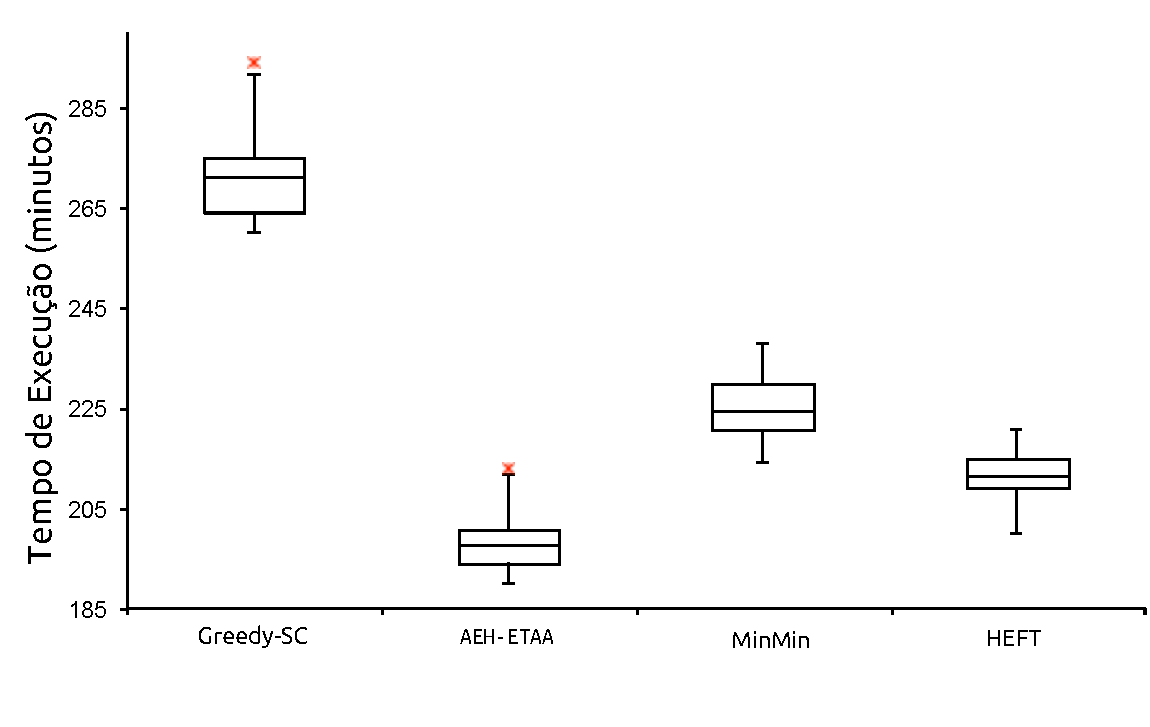
\includegraphics[width=.8\linewidth]{figure/Graphic_FGCS.pdf}
\caption{Diagrama de caixa comparando as execuções do SciPhy utilizando os algoritmos de escalonamento AEH-ETAA, Greedy-SC, HEFT e MinMin.}
\label{fig:boxplot}
\end{figure}



A Tabela \ref{tabelaEstimativa}, apresenta a média dos valores de \textit{makespan} estimados pelos algoritmos estáticos (MinMin, HEFT e AEH-ETAA) em comparação com os valores reais obtidos na execução. Note que os algoritmos estimaram tempos menores em relação aos tempos reais obtidos, representando uma diferença média de mais ou menos $26\%$. Isso ocorre pois tanto os \textit{overheads} oriundos do SciCumulus (como o tempo de consulta à base de dados, por exemplo), quanto as variações de performance das MVs, não são consideradas pelos algoritmos estáticos. Os valores de tempo estimado do algoritmo Greedy-SC não são apresentados, pois como se trata de um algoritmo dinâmico, não há uma estimativa prévia dos tempos de execução do \textit{workflow} escalonado pelo Greedy-SC.
% Todas os valores estatísticos das execuções (mediana, valor minimo, valor máximo, primeiro quartil, terceiro quartil e média) são apresentados na Tabela \ref{resultsciphy}. 


\begin{table}[H]
\small
\begin{center}
\caption{Comparação dos valores estimados e obtidos pelos algoritmos de escalonamento.}
\label{tabelaEstimativa}
\begin{tabular}{|c|c|c|}
\hline
\textbf{Algoritmo} & \textbf{Tempo Estimado} & \textbf{Tempo obtido} \\
\hline
\hline
Greedy-SC   &  \textbf{--} & 273,1\\
MinMin      & 219,31 & 224,6 \\ 
HEFT        & 168,10 & 214,5\\
AEH-ETAA    & 133,36 & 198,2\\
\hline
\end{tabular}
\end{center}
\end{table}	







% This subsection presents the execution time of SciPhy using a greedy scheduling algorithm \cite{Oliveira2012}, MinMin-TSH, HEFT and HEA-TaSDAP scheduling plans in SciCumulus system. The results are presented in Figure \ref{fig:boxplot}. SciPhy was executed 5 times for each approach in order to achieve statistical significance.
% As presented in Figure \ref{fig:boxplot}, the total execution time of SciPhy when using greedy scheduling was of 273.1 minutes in average, was of 224.6 minutes when using MinMin-TSH, was of 214.5 and when using HEA-TaSDAP was of 198.2 minutes in average.
% It represents approximately 27.4\% of improvement when using HEA-TaSDAP in comparison with the greedy algorithm of SciCumulus, 11.7\% of improvement in comparison with MinMin-TSH and 8.1\% of improvement in comparison with HEFT. This difference is due to the data file assignment of HEA-TaSDAP. Most of the bigger data files were placed in VMs with high bandwidth. In case of greedy scheduling and MinMin-TSH, some data files with several GB were placed in VMs with low bandwidth. It is worth mentioning that although HEA-TaSDAP estimated the total execution time in 133.36 minutes, it did not consider variations in the VM performance (which is expected in the cloud environment), the time needed to deploy the VMs in Amazon EC2, to start SciCumulus engine in all VMs involved in the execution and the implicit overhead of querying the database to discover the tasks to execute (~2\% of the total execution time of the workflow).



% In addition, in the execution with the greedy scheduling approach, all data is synchronized for all 3 VMs using Amazon S3, which implies in a certain overhead for every data file produced.
% The overall statistics of the execution (median, min, max, Quartile 1, Quartile 3 and Average) are also presented in Table \ref{resultsciphy}. It is worth noticing that there were no failures neither performance variations in the VMs during the workflow execution. If there were failures or performance variations, the execution using HEA-TaSDAP, HEFT and MinMin-TSH would probably produce worse results since they consider a static set of VMs during the entire execution. Nevertheless, the results are promising and more tests are planned using different workflows such as Montage and Ligo.

% \begin{table}[H]
% \small
% \begin{center}
% \caption{Valores estimados pelos algoritmos de escalonamento}
% \label{resultsciphy}
% \begin{tabular}{|c|c|c|c|c|c|c|}
% \hline
% \textbf{Algoritmo} & \textbf{Média} & \textbf{Mediana} & \textbf{Min} & \textbf{Max} & \textbf{Q1} & \textbf{Q3} \\
% \hline
% \hline
%         Greedy-SC  & 273,1          & 271,0            & 260,3        & 295,9        & 264,1       & 275,2 \\ 
%         AEH-ETAA   & 198,2          & 198,7            & 190,3        & 213,2        & 194,4       & 201,8 \\
%         HEFT       & 214,5          & 211,5            & 198,5        & 221,7        & 209,5       & 215,2 \\
%         MinMin     & 224,6          & 224,6            & 214,2        & 238,0        & 221,9       & 230,6  \\ 
% \hline
% \end{tabular}
% \end{center}
% \end{table}	





% \begin{table}[H]
% \centering
% \caption{Resultados das execuções do SciPhy - Valores em minutos}
% \label{resultsciphy}
% \begin{tabular}{@{}lllllll@{}}
% \hline 
% \toprule
% Approach & Average & Median & Min & Max & Q1 & Q3 \\ \midrule
% \hline 
% Greedy & 273.1 & 271.0 & 260.3 & 295.9 & 264.1 & 275.2 \\ \midrule
% HEA-TaSDAP & 198.2 & 198.7 & 190.3 & 213.2 & 194.4 & 201.8 
% \\ \midrule
% HEFT & 214.5 & 211.5 & 198.5 & 221.7 & 209.5 & 215.2 
% \\ \midrule
% MinMin-TSH & 224.6 & 224.6 & 214.2 & 238.0 & 221.9 & 230.6  \\ \bottomrule
% \end{tabular}
% \end{table}

